%%%%%%%%%%%%%%%%%%%%%%%%%%%%%%%%%%%%%%%%%
% University/School Laboratory Report
% LaTeX Template
% Version 3.1 (25/3/14)
%
% This template has been downloaded from:
% http://www.LaTeXTemplates.com
%
% Original author:
% Linux and Unix Users Group at Virginia Tech Wiki 
% (https://vtluug.org/wiki/Example_LaTeX_chem_lab_report)
%
% License:
% CC BY-NC-SA 3.0 (http://creativecommons.org/licenses/by-nc-sa/3.0/)
%
%%%%%%%%%%%%%%%%%%%%%%%%%%%%%%%%%%%%%%%%%

%----------------------------------------------------------------------------------------
%	PACKAGES AND DOCUMENT CONFIGURATIONS
%----------------------------------------------------------------------------------------

\documentclass{article}

\usepackage{siunitx} % Provides the \SI{}{} and \si{} command for typesetting SI units
\usepackage{graphicx} % Required for the inclusion of images
\usepackage[utf8]{inputenc}
\usepackage{natbib} % Required to change bibliography style to APA
\usepackage{amsmath} % Required for some math elements
\usepackage{mathtools}
\renewcommand{\refname}{Bibliografia}
\renewcommand{\contentsname}{Indice}

\setlength\parindent{0pt} % Removes all indentation from paragraphs

\renewcommand{\labelenumi}{\alph{enumi}.} % Make numbering in the enumerate environment by letter rather than number (e.g. section 6)

%\usepackage{times} % Uncomment to use the Times New Roman font

%----------------------------------------------------------------------------------------
%	DOCUMENT INFORMATION
%----------------------------------------------------------------------------------------

\title{Modellazione della microcircolazione retinica\\tramite analogia fluido - elettrica} % Title

\author{Giulio Gargantini} % Author name

\date{Ottobre 2019} % Date for the report

\begin{document}

\maketitle % Insert the title, author and date

\begin{center}
Prof. A.G. Mauri \\
Computational Models for Electronics and Biomathematics\\
Politecnico di Milano\\
A.A. 2018/2019
\end{center}

% If you wish to include an abstract, uncomment the lines below
\begin{abstract}
In questo progetto si è voluto simulare la microcircolazione nella retina modellandola come un circuito elettrico a resistenze variabili con l'obiettivo di replicare i risultati di \cite{art1}.
L'attenzione è rivolta in particolare alla stima del flusso sanguigno nella microcircolazione per individui aventi valori diversi di pressione sanguigna e pressione intraoculare.
\end{abstract}

\tableofcontents
\newpage
%----------------------------------------------------------------------------------------
%	INTRO
%----------------------------------------------------------------------------------------

\section{Introduzione}
Nello studio della fisiologia dell'apparato visivo e nella ricerca relativa ad alcune sue disfunzioni, una buona comprensione della microcircolazione sanguigna a livello della retina riveste un ruolo fondamentale.
La retina è irrorata da una rete di vasi esposti alla pressione interna del bulbo oculare, la quale può, se alterata, inibire un corretto afflusso di sangue e favorire l'insorgenza di patologie come il glaucoma.
Vista l'importanza cruciale dell'individuazione delle cause precise di una malattia tanto invalidante, i ricercatori si sono concentrati sullo sviluppo di modelli capaci di simulare in modo efficace la microcircolazione retinica e le sue interazioni con la struttura dell'occhio.

Il modello su cui si concentra questo progetto è presentato in \cite{art1} e sfrutta l'analogia elettrico-idraulica (cfr. capitolo 4 di \cite{notes}) per modellare la rete di vasi sanguigni come un circuito elettrico a resistenze variabili.
Ciò permette di prendere in considerazione l'azione della pressione intraoculare (IOP) e della pressione sanguigna sulla larghezza dei vasi, strettamente correlata alla resistenza idraulica degli stessi e al flusso di sangue complessivo in un ciclo cardiaco.

Questo rapporto si articola in quattro parti principali.
Nella prima si illustra il quadro generale del problema partendo dall'anatomia e fisiologia delle porzioni dell'occhio analizzate, per poi procedere, nella seconda parte, alla deduzione di un modello ridotto della microcircolazione secondo l'analogia fluido-elettrica.
Nella terza si illustra l'implementazione del modello ricavato nella sezione precedente tramite un codice Matlab e si presentano le relazioni principali tra le diverse funzioni.
Infine la quarta parte è dedicata ai risultati ottenuti e al confronto con quelli ottenuti in \cite{art1}, discutendone il significato fisico e l'importanza.

%----------------------------------------------------------------------------------------
%	SECTION 1
%----------------------------------------------------------------------------------------

\section{Anatomia e fisiologia}
In questa sezione si descrivono le componenti dell'occhio che vengono studiate nel modello in esame.
\begin{figure}[h]
\begin{center}
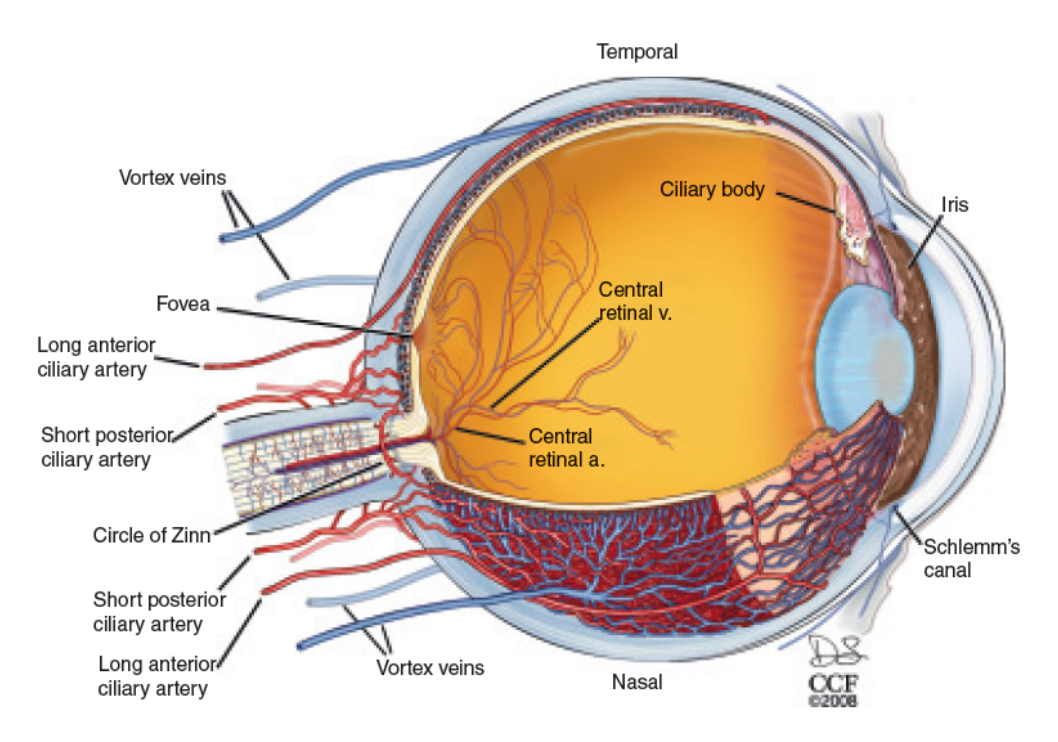
\includegraphics[width=0.8\textwidth]{Pictures/occhio.png}
\caption{Struttura generale dell'occhio \cite{Tesi}}
\label{eyeball}
\end{center}
\end{figure}
L'occhio ha una forma grossomodo sferica, la cui porzione centrale è occupata dall'umore vitreo, una sostanza gelatinosa e trasparente che mantiene la tonicità del globo oculare. 
L'umor vitreo è completamente racchiuso dalla sclera, una membrana di tessuto fibroso di colore bianco, ad eccezione della parte anteriore in cui esso è limitato dal cristallino.
Tra il cristallino e la cornea, la membrana trasparente che separa l'occhio dall'esterno, si trovano due sezioni, dette camera anteriore e posteriore, separate dall'iride e contenenti l'umor acqueo.

Sulla parte posteriore dell'occhio, adagiata sulla sclera, si trova la retina: un tessuto fotosensibile capace di trasformare i segnali luminosi in impulsi nervosi i quali, raccolti dal nervo ottico, vengono inviati al cervello \cite{Tesi}.
\subsection{Anatomia della retina}
A differenza della sclera, irrorata da molteplici vasi sanguigni come le arterie e le vene ciliari e le vene vorticose, gli unici collegamenti tra la rete di capillari della retina e il flusso sanguigno sono l'Arteria Retinica Centrale (CRA) e la Vena Retinica Centrale(CRV).
\begin{figure}[h]
\begin{center}
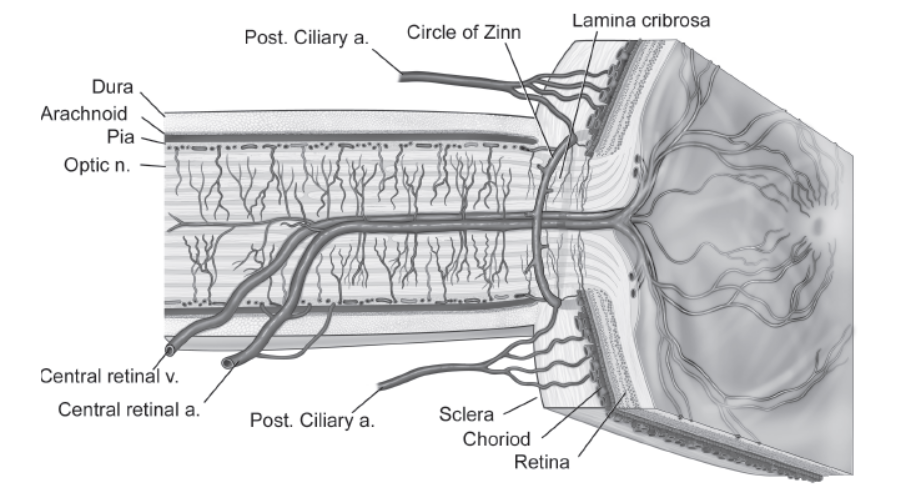
\includegraphics[width=0.8\textwidth]{Pictures/Optic_nerve.png}
\caption{Principali vasi retinici \cite{Tesi}}
\label{retina}
\end{center}
\end{figure}
Entrambi i vasi percorrono un tratto all'interno del nervo ottico, circondati dalle fibre nervose e entrano nell'occhio attraverso la Lamina Cribrosa: tale lamina è una porzione della sclera forata in molteplici punti, attraverso la quale passano le fibre innervanti la retina, la CRA e la CRV (cfr. figura \ref{retina}).
A questo punto l'arteria centrale si divide in molteplici arteriole e capillari, i quali, dopo aver irrorato le cellule della retina, si ricongiungono formando una rete di venule che, a loro volta, si uniscono nella CRV.

I vasi sanguigni non hanno pareti rigide, quindi la loro sezione è soggetta a variazioni dovute alla differenza tra la pressione esterna e interna al vaso: nella zona del nervo ottico i vasi sono soggetti alla pressione del tessuto retrolaminare (RLTp) mentre all'interno del bulbo oculare sono esposti alla pressione intraoculare (IOP).
Vene e arterie sono costituite da tessuti diversi e hanno una diversa struttura: le prime sono generalmente più fini delle seconde e devono sostenere una pressione interna più debole.
Per questo motivo esse sono più soggette ad ampie variazioni di volume e al rischio di collassare su loro stesse se la pressione interna non è in grado di controbilanciare quella agente sulle pareti della vena.
\subsection{Circolazione dell'umor acqueo}
La pressione interna dell'occhio (IOP) è mantenuta grazie alla produzione di umor acqueo.
Questo liquido trasparente simile al plasma è prodotto dal corpo ciliare nella camera posteriore dell'occhio, da cui filtra nella camera anteriore attraverso l'iride e la pupilla.
Dalla camera anteriore esso passa attraverso il trabecolato, una struttura porosa posta tra la sclera e la cornea, per esser drenato nel canale di Schlemm per disperdersi infine nella circolazione venosa (cfr. figura \ref{umoracqueo}).
\begin{figure}[h]
\begin{center}
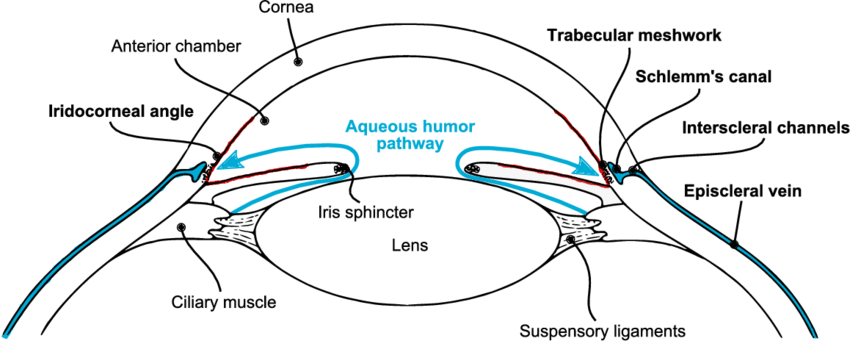
\includegraphics[width=0.8\textwidth]{Pictures/umor_acqueo.png}
\caption{Circolazione dell'umor acqueo nelle camere posteriore e anteriore \cite{Tesimmagine}}
\label{umoracqueo}
\end{center}
\end{figure}
Nel caso in cui non si verifichi un normale drenaggio dell'umor acqueo, ad esempio per l'occlusione del trabecolato, il fluido si accumula nella camera anteriore dell'occhio premendo sul cristallino e trasmettendo la pressione all'umor vitreo, aumentando così l'IOP.
Tale aumento della pressione esterna può provocare il collasso dei vasi sanguigni della retina, in particolare delle vene, diminuendo l'irrorazione  del tessuto e favorendo l'insorgenza del glaucoma.

Per contrastare gli effetti di un'elevata IOP è stata sviluppata la trabeculectomia: un'operazione chirurgica in cui si effettua un foro nella sclera in corrispondenza della camera anteriore, permettendo all'umor acqueo di drenare in una sacca al di sotto  della congiuntiva.
Permettendo nuovamente il drenaggio del fluido si osserva una considerevole riduzione del valore dell'OPP nei pazienti, riportandolo ai livelli fisiologici (cfr. tabela 6 di \cite{art1}).

\section{Derivazione del modello}
\subsection{Analogia fluido - elettrica}
Nel capitolo 4 di \cite{notes} si presenta in dettaglio l'analogia fluido - elettrica, ovvero come una rete di tubi percorsi da un fluido incomprimibile si possa descrivere con le stesse equazioni cusate per modellare i circuiti elettrici.
Si consideri il flusso come l'analogo della corrente e la pressione del fluido corrispondente al potenziale elettrico in un punto del circuito.
Sotto quest'analogia si osserva che la caduta di pressione ai due capi di un tubo si può interpretare come l'effetto di una resistenza idraulica e le proprietà elastiche di una sezione della rete, che permettono a una porzione del vaso di accumulare il fluido, si possono ricondurre agli effetti capacitivi di un condensatore.
Inoltre si può mostrare che le leggi di Kirchhoff per il potenziale e per la corrente sono ugualmente valide in questo contesto.

Senza ripetere i calcoli che portano a definire l'analogia fluido - elettrica, si riportano nella tabella \ref{tab_analogia} le equivalenze tra le grandezze principali e le unità di misura utilizzate.

\begin{table}[h!]
\begin{center}
\begin{tabular}{| c | c |}
\hline
\textbf{Grandezza elettrica} & \textbf{Grandezza idraulica}\\
\hline
Tensione [\si{\volt}] & Pressione [\si{\mmHg}]\\
Corrente [\si{\ampere}] & Flusso [\si{\milli\liter \per \minute}]\\
Carica [\si{\coulomb}] & Volume [\si{\milli\liter}]\\
Resistenza elettrica [\si{\ohm}] & Resistenza idraulica [\si{\mmHg \second \per \milli\liter}]\\
Capacità elettrica [\si{\farad}] & Capacità idraulica [\si{\milli\liter \per \mmHg}]\\
\hline
\end{tabular}
\caption{Confronto tra grandezze equivalenti nell'analogia fluido - elettrica e corrispondenti unità di misura}
\label{tab_analogia}
\end{center}
\end{table}


\subsection{Deduzione del circuito}
I vasi della microcircolazione retinica si possono dividere in cinque compartimenti: la CRA, le arteriole, i capillari, le venule e la CRV numerati da $1$ a $5$.
Ciascun compartimento può essere diviso in sezioni rappresentanti le diverse porzioni dei vasi e ciascuna di esse è modellata come un resistore in un circuito elettrico.
Ogni resistore è identificato dal numero del compartimento corrispondente e da una lettera.
Essendo le pareti dei vasi sanguigni elastiche, vene e arterie possono variare il loro volume e immagazzinare del sangue nel corso del ciclo cardiaco: tale proprietà è descritta da una capacità assegnata ad ogni compartimento ed è rappresetata nel modello circuitale tramite dei condensatori.

\begin{figure}[h]
\begin{center}
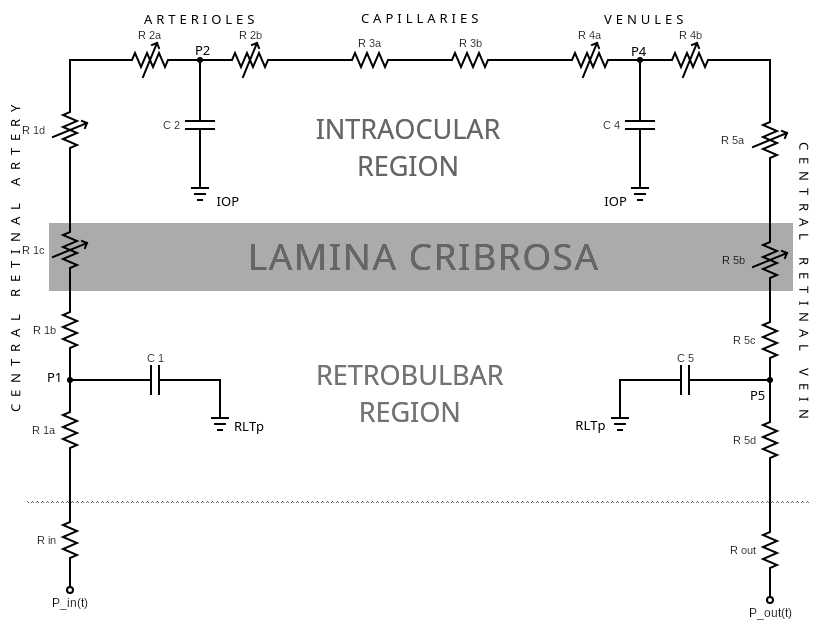
\includegraphics[width=1.0\textwidth]{Pictures/circuit1.png}
\caption{Rappresentazione circuitale della microcircolazione retinica \cite{art1}}
\label{circuito}
\end{center}
\end{figure}

Il modello adottato in \cite{art1} rappresenta la microcircolazione retinica tramite il circuito rappresentato nella figura \ref{circuito}.
La CRA e la CRV sono gli unici vasi che attraversano la lamina cribrosa passando dal nervo ottico alla regione intraoculare.
Per questo motivo tali compartimenti sono rappresentati tramite quattro resistori: due per la regione retrobulbare, uno per la porzione di vaso che attraversa la lamina cribrosa e uno per la regione intraoculare.
Le sezioni dei vasi nella regione retrobulbare sono sottoposte alla pressione del tessuto retrolaminare (RLTp), la porzione all'interno dell'occhio è sottoposta alla pressione intraoculare (IOP) mentre la pressione esercitata dalla lamina cribrosa è modellata seguendo il modello descritto in \cite{art3} e descritta in una sezione dedicata.
La sezione nella regione retrobulbare è divisa in due resistori per ciascun vaso ($R_{1a}$, $R_{1b}$ e $R_{2a}$, $R_{2b}$ rispettivamente) in modo che i corrispondenti condensatori $C_1$ e $C_5$ agiscano sulla pressione media dei vasi nel nervo ottico.

I compartimenti delle arteriole, capillari e venule sono modellati tramite due resistori ciascuno.
Arterie e venule sono modellate tramite i condensatori $C_2$ e $C_4$ connessi in modo tale che le proprietà capacitive agiscano sulle pressioni medie in ciascuno dei compartimenti.
Non essendo i capillari dotati di pareti elastiche, la sezione corrispondente non è connessa ad alcun condensatore.

Le pressioni $P_{in}$ e $P_{out}$ agli estremi del circuito sono funzioni del tempo  ricavate dalla figura 3c di \cite{art1} e rappresentano le pressioni sanguigne arteriosa e venosa rispettivamente a monte e a valle della microcircolazione; la connessione tra le pressioni in input e il circuito è effettuata tramite i resistori $R_{in}$ e $R_{out}$, rappresentanti i tratti di arteria e di vena prima della CRA e dopo la CRV.

Usando la legge di Kirchhoff per le correnti e la definizione di capacità, dal circuito si può ricavare il seguente sistema di equazioni differenziali ordinarie, la cui soluzione permette di ricavare l'evoluzione delle varie grandezze caratteristiche nel tempo e, in ultima analisi, dedurre il comportamento del sistema fisico.

\begin{equation}
\begin{dcases}
  C_1 \frac{d}{dt}(P_1 - RLT_p) &= \frac{P_{in} - P_1}{R_{in} + R_{1a}}  - \frac{P_1 - P_2}{R_{1b} + R_{1c} + R_{1d} + R_{2a}} \\
  C_2 \frac{d}{dt}(P_2 - IOP) &= \frac{P_1 - P_2}{R_{1b} + R_{1c} + R_{1d} + R_{2a}}  - \frac{P_2 - P_4}{R_{2b} + R_{3a} + R_{3b} + R_{4a}} \\
  C_4 \frac{d}{dt}(P_4 - IOP) &= \frac{P_2 - P_4}{R_{2b} + R_{3a} + R_{3b} + R_{4a}}  - \frac{P_4 - P_5}{R_{4b} + R_{5a} + R_{5b} + R_{5c}} \\
  C_5 \frac{d}{dt}(P_1 - RLT_p) &= \frac{P_4 - P_5}{R_{4b} + R_{5a} + R_{5b} + R_{5c}}  - \frac{P_5 - P_{out}}{R_{5d} + R_{out}}
\end{dcases}
\label{sistema}
\end{equation}
\subsection{Valore dei resistori}
\subsection{Pressione nella Lamina Cribrosa}

%----------------------------------------------------------------------------------------
%	SECTION 2
%----------------------------------------------------------------------------------------
\section{Codice}
%----------------------------------------------------------------------------------------
%	SECTION 3
%----------------------------------------------------------------------------------------
\section{Risultati}
%----------------------------------------------------------------------------------------
%	CONCLUSION
%----------------------------------------------------------------------------------------
\section{Conclusione}


\addcontentsline{toc}{section}{Bibliografia}
\bibliographystyle{unsrt}
\bibliography{sample}

%----------------------------------------------------------------------------------------


\end{document}